% -----------------------------------------------
% Template for ISMIR Papers
% 2025 version, based on previous ISMIR templates

% Requirements :
% * 6+n page length maximum
% * 10MB maximum file size
% * Copyright note must appear in the bottom left corner of first page
% * Clearer statement about citing own work in anonymized submission
% (see conference website for additional details)
% -----------------------------------------------

\documentclass{article}
\usepackage[T1]{fontenc}
\usepackage[utf8]{inputenc}
\usepackage{ismir} % Remove the "submission" option for camera-ready version
\usepackage{amsmath,cite,url}
\usepackage{graphicx}
\usepackage{color}

% Title. Please use IEEE-compliant title case when specifying the title here,
% as it has implications for the copyright notice
% ------
\title{TransVox: The Role of Digital Tools in Voice Training and the Development of a Gender-Diverse Speech Dataset}

% Note: Please do NOT use \thanks or a \footnote in any of the author markup

% Single address
% To use with only one author or several with the same address
% ---------------
\author{
    Isaiah Doyle\\University of Victoria\\\texttt{isaiahdoyle@uvic.ca}
}


% Two addresses
% --------------
%\twoauthors
%   {First author} {School \\ Department}
%   {Second author} {Company \\ Address}

%Three addresses
%--------------
% \author{
%    \textbf{Isaiah Doyle}\\ {University of Victoria \\\texttt{isaiahdoyle@uvic.ca}}
%    \and
%    \textbf{Aileen Klassen}\\ {University of Victoria\\\texttt{aileenklassen@uvic.ca}}
%    \and
%    \textbf{Elijah Larmer}\\ {University of Victoria \\\texttt{elijahlarmer@uvic.ca}}
% }

% Four or more addresses
% OR alternative format for large number of co-authors
% ------------
% \multauthor
%   {First author$^1$ \hspace{1cm} Second author$^1$ \hspace{1cm} Third author$^2$}
%   {{\bf Fourth author$^3$ \hspace{1cm} Fifth author$^2$ \hspace{1cm} Sixth author$^1$}\\
%   $^1$ Department of Computer Science, University, Country\\
%   $^2$ International Laboratories, City, Country\\
%   $^3$ Company, Address\\
%   {\tt\small CorrespondenceAuthor@ismir.edu, PossibleOtherAuthor@ismir.edu}
%   }

% For the author list in the Creative Common license, please enter author names.
% Please abbreviate the first names of authors and add 'and' between the second to last and last authors.
\def\authorname{I. Doyle}

% Optional: To use hyperref, uncomment the following.
% \usepackage[bookmarks=false,pdfauthor={\authorname},pdfsubject={\pdfsubject},hidelinks]{hyperref}
% Mind the bookmarks=false option; bookmarks are incompatible with ismir.sty.

\sloppy % please retain sloppy command for improved formatting

\begin{document}

\maketitle{}


\begin{abstract}
    Digital tools have made a significant impact on the state of vocal training for transgender individuals, from online communities to acoustic measurement tools. This latter group of digital tools tend to rely largely – or in many cases solely – on measurements of average fundamental pitch to determine the user's adherence to a particular gender ideal. Contemporary literature shows that our aural perception of gender is based on numerous other timbral characteristics that are not measured by applications on the market today. To accommodate the many parameters that factor into vocal perception, a program was proposed by Doyle et al. \cite{doyle2025} to resynthesize speech samples with applied timbral modifications, allowing users to train toward their preferred voice by vocal imitation. This paper outlines the role of digital tools in vocal training, then discusses further development of \cite{doyle2025}, and proposes the informed creation of a diverse speech dataset to improve the program's performance.
\end{abstract}


\section{Introduction}\label{sec:introduction}

Transgender (hereafter referred to as \textit{trans}) individuals may face voice-gender incongruence, motivating said individuals to seek a vocal timbre that more accurately reflects their desired gender expression. Voice training is widely considered to be an effective method for those seeking voice-gender congruence, ideally under the guidance of a speech-language pathologist (SLP) \cite{oates2023}.

Vocal training for trans people is distinct from traditional speech therapy in that its participants are unlikely to have a voice disorder, rather wishing to align particular features of their voice to those of a voice that is more likely to be perceived as their gender identity. This might look like a trans woman seeking a more feminine voice, a trans man seeking a more masculine voice, or those seeking a more flexible voice that does not strictly conform to either pole of binary gender.

While some trans people are able to seek the support of a SLP to explore the capabilities of their voice in an open environment, others opt toward a self-guided approach using advice from others in online communities \cite{kowalchuck2020} or applications designed to support voice training (e.g., \cite{devextras2018, nitzandseek2020, speechtools2013}), due to the accessibility of digital tools.

The satisfaction of individuals undergoing voice training depends on habitual timbral characteristics in addition to average pitch and pitch range. However, modern applications designed to support voice training \cite{devextras2018, nitzandseek2020, speechtools2013} tend to rely on fundamental pitch as the primary measure of progress. While pitch is certainly a factor in the perception of gender through the voice, other timbral aspects of the voice are also critical in expressing a particular gender identity. For this reason, digital tools that favour pitch over all other timbral parameters fail to deliver the same comprehensive feedback that regular instruction from a SLP would be capable of.

While no comprehensive structured program for voice training exists, current programs commonly begin with foundational training to promote vocal health and flexibility before moving on to realize specific timbral goals \cite{oates2023}. The latter vocal transformation stage can look a number of ways; one such strategy, once initial vocal manipulation skills are mastered, is vocal imitation. In the imitation model, SLPs will either use their own voice to demonstrate vocal techniques to their clients or use a recording a voice demonstrating some target. The client is then expected to imitate the target voice to the best of their ability using techniques taught by the SLP.

Although vocal imitation is an effective method of habitual learning (particularly when delivered alongside detailed techniques from a SLP) \cite{ohlsson2024}, the SLP-driven or recording-driven target may fail to reflect the distinct properties of the participant's voice like accent or prosody, adding a level of guesswork to the imitation process. With this in mind, Doyle et al. \cite{doyle2025} sought to develop a proof-of-concept for a program capable of converting a speech sample from a \textit{source} voice into a \textit{target} voice that retains the fundamental characteristics of the speech sample but modifies timbral characteristics relating to aural perception of gender. With a customizable voice model, users would be able to explore the timbral possibilities of their voice and create more clearly defined training goals that can be practiced via imitation.

Some changes were made to the program in \cite{doyle2025}, and further work is necessary to improve the program's accessibility. In the long run, we anticipate this being a component of a larger application designed to support SLPs and individuals developing their unique preferred vocal timbre.

This document first outlines some commonly agreed-upon goals for voice training, and how digital tools currently approach individually-driven practice. Then a summary of \cite{doyle2025} is provided alongside advancements made to the project. Finally, a plan is proposed for the creation of a safe and informed gender-diverse speech dataset to improve the performance of the program.

\section{Digital Tools for Vocal Training}

The goal of vocal training for trans individuals is to work toward habitual voice-gender congruence, which, for some, may look like conforming to a particular pole of the socially traditional gender binary (i.e., a masculine or feminine voice). For others, vocal training may be more open-ended, instead acting as an exploration into the capabilities of one's voice and seeking an oral expression that reflects their gender identity.

Although there is no specific, standardized guide for voice training available, commonly targeted characteristics associated with the perception of gender are pitch and pitch range, resonance, intensity, breathiness, and articulation \cite{coleman2022, leyns2021, oates2019, oates2023, davies2015}. While many of these can be measured objectively, each individual approaches voice training with special circumstances that make generalization of a single training program impossible. Ideally, each person seeking vocal transformation would adhere to a personalized training plan suggested by a professional SLP.

Coleman et al. \cite{coleman2022} define standards of care to guide health care professionals in supporting trans and gender diverse (TGD) people. The term TGD is used throughout the guide to include a diverse range of gender identities, and the authors make a number of recommendations with all TGD people in mind. Importantly, the authors discuss the difficulties that TGD people face when seeking help with regard to vocal training, especially those with intersectional marginalized identities. A significant margin of TGD people wish to partake in voice training, but lack the means to access quality professional support.

The rise of digital technology has made a significant difference in the ecology of voice training due to its monetary and social accessibility. There are a number of free and paid smartphone applications available that are being used to help individuals practice voice training both alone and in community, with some of the more targeted applications claiming to be the "next best thing" to support from a registered SLP \cite{devextras2018, nitzandseek2020, speechtools2013}. These tools are incredibly important in improving the accessibility of voice training for TGD individuals, but raise concerns with respect to vocal health and inclusivity.

While some more in-depth applications like \cite{speechtools2013} seek to emulate guided support from a SLP including foundational skills, other applications provide limited metrics \cite{devextras2018, nitzandseek2020} that risk being misused by its users if foundational skills are not already developed.

Additionally, many of these digital tools seek to generalize the vocal training process for all users due to the limited capacity of smartphone applications. Most of these apps categorize gender identities into strict objectively measurable categories, which is convenient for app developers, but often fails to recognize the needs of all TGD people, especially those with otherwise marginalized identities \cite{ahmed2022}.

Voice training should be an informed exploration of one's own vocal capabilities, which can be difficult to do on one's own, especially when an app designed to help is leading them toward a goal that does not align with their ideal voice or fails to recognize their intersectional identities.


\section{TransVox}\label{sec:page_size}

TransVox is a tool introduced by Doyle et al. \cite{doyle2025} to support the vocal imitation strategy sometimes used during voice training to practice techniques taught by a SLP. This project is not intended to serve as a standalone method for voice training, but may serve as a useful imitation tool once rigorous foundational skills are established.

The program functions by receiving a speech sample of any length alongside desired values for breathiness, pitch, smoothness, and tone. The program then resynthesizes the input sample with the selected timbral parameters, resulting in a copy of the speech sample with a different vocal timbre.

The following section summarizes the findings of \cite{doyle2025}; then, the steps taken from May to August 2025 to advance the project are discussed.

\subsection{Previous Work}

The program utilizes an existing framework for voice conversion called FreeVC \cite{li2022}, which is capable of extracting either a mel-spectrogram or speaker encoder representation of the timbre of a \textit{target} voice (i.e., a \textit{timbre vector}) alongside the content representing words spoken by a \textit{source} voice. The content and timbre are then combined to synthesize a new speech sample using the content of the source voice and the the timbre of the target voice. This occurs in a two-step process such that the timbre vector is exposed before resynthesis, allowing for timbral modification by operating on the vector directly. In the case of TransVox, both the source and target voices are the same speech sample, allowing the speech sample to be effectively cloned with or without timbral modification.

A 900-file subset of Mozilla's Common Voice Corpus Delta Segment 21.0 \cite{mozilla2025} was selected and manually stripped of any unsuitable data, resulting in a dataset of 657 samples. A script was then created to allow the developers to rate each sample from 1 to 5 according to perceived levels of breathiness, pitch, smoothness, and tone. For each sample, labels were derived by taking the averages of the developers' ratings for each parameter.

Trends were derived from the dataset by grouping the samples by their ratings and making a generalized timbre model for each segment by averaging the timbre representations of all speech samples within. Analysis of these trends was promising, particularly on the scale of pitch which showed significant polarization in the generalized timbres for the low and high segments. Several methods were attempted to apply these trends to mel-spectrograms, the most effective of which involved dividing the dataset into four groups according to their rating for pitch and taking the average MFCC difference of the input sample's expected grouping from the other three groups. A model was attempted to be trained on the dataset with the goal of automatically situating input samples into a group, but accuracy scores were low across the board for both Gaussian Naive Bayes (GNB) and Random Forest (RF) classifiers.

Results were thus varied, and relied on the manual classification of an input sample into its expected group. Resulting audio samples can be found in the associated GitHub repository \cite{github} alongside usage information.


\subsection{Progression}

\begin{figure}
    \centering
    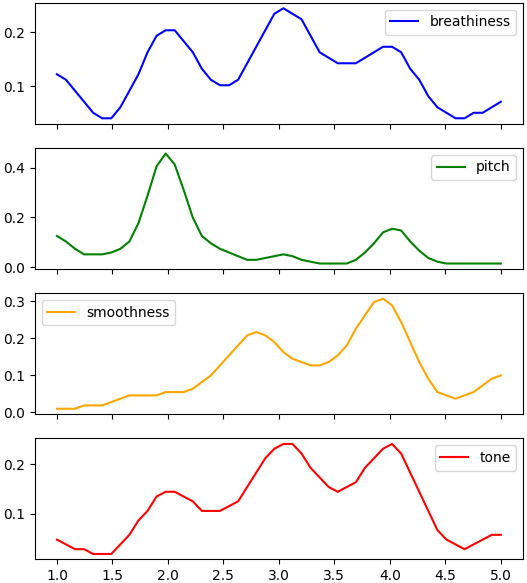
\includegraphics[width=0.9\linewidth]{distributions.png}
    \caption{Distribution of sample ratings for breathiness, pitch, smoothness, and tone}
    \label{fig:distributions}
\end{figure}

The most significant drawbacks of \cite{doyle2025} lie in the model's fragility when recreating voices that lie \textit{between} the poles of traditionally masculine and feminine. These more androgynous voices tend to exhibit timbral artifacts that jump between the two poles rather than maintain a significant intermediate version. These "middle" voices are crucial for presenting a gradual sequence of voices between targets of an opposite pole, as well as accommodating users that have timbral targets that lie outside the traditional gender binary.

Initial considerations involved the creation of a \textit{comparative} dataset, which would leverage differences in voices before and after modification, rather than generalized differences between a large number of speakers, to train a model on how a voice might change over time. Though potentially still useful, a comparative dataset would likely still lead to the problems above, as comparing two voices still leaves out the intermediate steps between them.

The scale of pitch shows a considerable gap in samples around its centre, with the majority of samples being situated around values of 2.0 or 4.0, indicating a majority of perceptually male and female voices. \figref{fig:distributions} illustrates this relatively low number of samples around the 3.0 rating, which may contribute to the model struggling to synthesize voices that lie between the low and high poles with regard to pitch.

Using an any-to-any model instead of FreeVC (many-to-many) was also considered due to a hypothesis that FreeVC may not be capable of generating androgynous voices because of a lack of available samples to pull from in the dataset. However, this was put into question by an informal examination of the model's ability to resynthesize androgynous voices without modification. Results were fairly successful for simple voice replication, but were not always to the same quality as more polarized voices. While this was being considered, focus was directed toward the modification of timbre vectors to truly determine if it would be possible to convert a perceptibly male or female voice to one that lies in between those two poles.

% The idea of a new \emph{comparative} dataset was proposed, which would leverage differences in voices before and after modification, rather than generalized differences between a large number of speakers, to train a model on timbre representations.

Using both mel-spectrogram and speaker encoder representations of timbre, a number of approaches were attempted to experiment with controlling the intermediate timbre vectors to affect parameters like pitch or breathiness. Focus was placed on using the same FreeVC-based analyze-modify-synthesize pipeline as \cite{doyle2025}, but instead of using generalized timbres pulled from the original dataset, experimenting with different methods for manipulating the timbre representations directly.

One such method involved applying pitch and formant shifting to the input audio before sending it through the speaker encoder. \figref{fig:mel-shift} shows a clear correspondence between the original timbre and its respective shifts of 1.5x and 2.0x the original pitch, both with lifter quefrencies of 3 milliseconds corresponding to the same amount of formant shifting. The original mel-spectrum $T_m$ (taken by averaging over the whole spectrogram) is stretched for each subsequent shift, while generally maintaining its original contour. The same process applied to FreeVC's speaker encoder representation $T_s$ in \figref{fig:spk-shift} is less observable as a latent space, but both $T_m$ and $T_s$ yield similar results once synthesized.

Using both $T_m$ and $T_s$ to synthesize the resulting timbre after pitch shifting led to quality voice conversion between the source speaker and a single potential target speaker -- that is, a voice that resembles the source timbre in quality but differs with respect to gender perception. However, attempts to generate intermediate steps between gender poles faced the same issues as above. In every case, the perceptual quality of using $T_s$ to synthesize output is better than $T_m$ despite suffering the same issues with intermediate voices. Further iterations then opted for using speaker encoder timbre vectors over mel-spectrograms.

Since it is possible to create a believable fully transitioned voice in the current state of the project, attempts were made to interpolate between the source timbre representation and a generated target timbre using both linear interpolation and ridge regression. Both attempts were also unsuccessful in the same way, suggesting that a more robust method for detecting trends is required to effectively model the nonlinearity of a voice in transition.

\begin{figure}
    \centering
    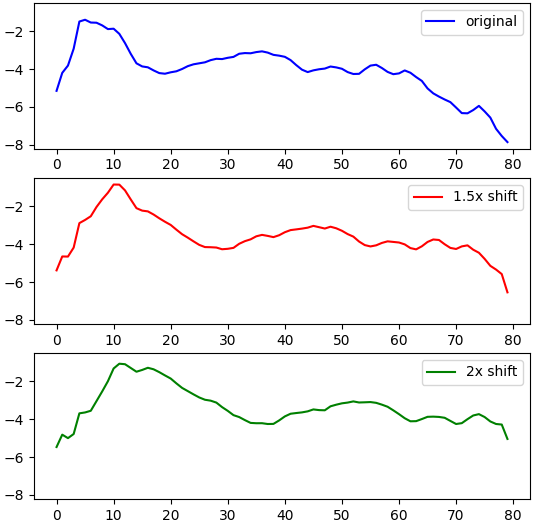
\includegraphics[width=0.9\linewidth]{mel-shift.png}
    \caption{Effects of pitch shifting on generalized mel-spectra $T_m$}
    \label{fig:mel-shift}
\end{figure}

\begin{figure}
    \centering
    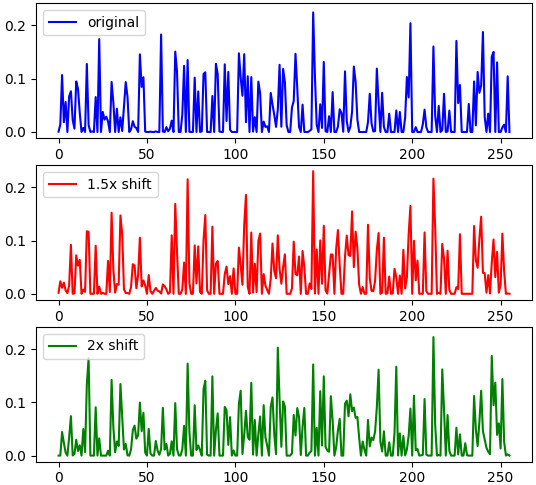
\includegraphics[width=0.9\linewidth]{spk-shift.png}
    \caption{Effects of pitch shifting on generalized speaker encoder representations $T_s$}
    \label{fig:spk-shift}
\end{figure}

One such method for creating a diverse range of voices is employing a generative model capable of mapping between voices in a nonlinear way. A variational autoencoder (VAE) is a generative version of an autoencoder with the ability to create new samples that resemble training data without imitating the data directly \cite{kingma2013}. A \textit{conditional} VAE (CVAE) allows for the conditioning of said generated output, leaning the result toward a particular label \cite{sohn2015}. It was hypothesized that if a timbre vector can be sent through a CVAE's encoder to yield a lower-dimensional representation, the decoder can then be conditioned to convert that lower-dimensional representation back into a full timbre vector, but breathier, or with higher pitch, for example.

In this case, the input to the CVAE's encoder is a 256-float array representing FreeVC's speaker encoder timbre vector $T_x$, and a condition vector $c$ representing its perceptual timbral parameters (e.g., pitch, breathiness, etc.). The encoder then reduces the dimensions of $T_x$ to create a lower-dimensional representation $T_z$. In training, the decoder takes $T_z$ and $c$ as input to recreate $T_x$ to the best of its ability. In practice, a CVAE can be used to randomly sample $T_z$ from a probability distribution to generate a completely new timbre $T_y$ corresponding to the supplied condition $c$, thus disregarding the encoder during inference.

The same dataset from \cite{doyle2025} was used to train the CVAE with 6-10 epochs. Each training epoch takes the first 500 samples in the dataset in batches of roughly 80, and uses the final 157 samples for testing. The loss value from the first batch in the first epoch was around 181 and decreased logarithmically as seen in \figref{fig:training-loss}, to converge around a loss value of approximately 36 after only the first few epochs.

After some experimentation, the CVAE model proved effective as a means for cloning and transforming timbres but still struggles to convert traditionally masculine or feminine voices into a more androgynous range. Referring back to the distribution of pitch ratings in \figref{fig:distributions}, this is likely due to a significant lack of samples around the pitch rating of 3.0 (i.e., androgynous-leaning voices).

The CVAE model lends itself well to intuitive interaction, as the only user-supplied parameters for the encoder and decoder are the condition vectors. Another advantage of the CVAE method is how easily one can make randomly varied voices by arbitrarily modifying some of the other timbral parameters. The same condition vector is currently being given to both the encoder and decoder, which may not be ideal since the encoder condition is intended to represent the perceptual qualities of the input and the decoder condition the qualities of the output, which should contrast. With a more comprehensive dataset like the one called for in \cite{doyle2025}, an improved classifier can be trained to estimate the encoder condition, potentially leading to more effective decoding.

\begin{figure}
    \centering
    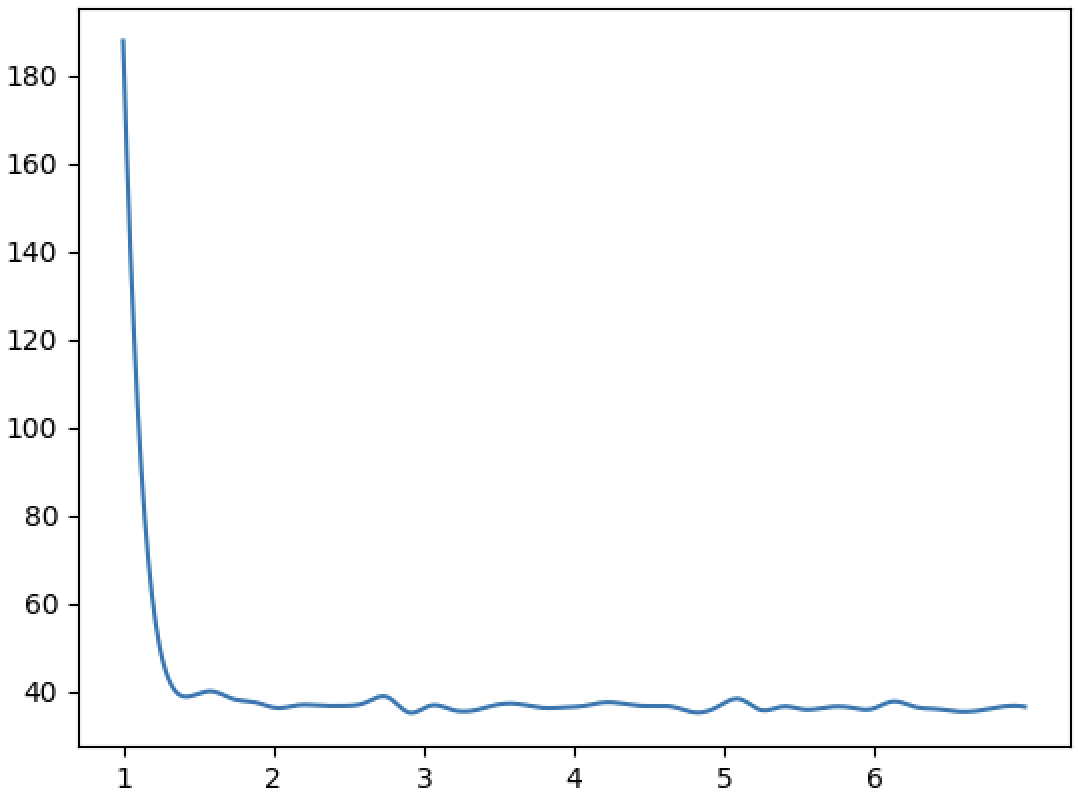
\includegraphics[width=0.9\linewidth]{training-loss.png}
    \caption{Impact on training loss for the first six epochs}
    \label{fig:training-loss}
\end{figure}


\section{Future Work}

% Besides the base functionality of the program, a simple user interface (UI) is also to be designed, allowing non-developers to use and test the program accordingly when the time for beta testing arrives. For effective development of the program as a whole, some consultation is necessary with professional voice coaches and members of the Trans + community. Hearing from individuals with intimate experience in the field will be paramount to creating a truly valuable tool for those undergoing vocal training, gathering information about its perceived social impacts and effectiveness as a training tool. It's critical that this project be approached with sensitivity, and an understanding of the ethics of the synthesis of queer voices \cite{sigurgeirsson2024}.

The limitations imposed by the current state of the project all point toward the shortcomings of the dataset used to train the CVAE, and likely also the FreeVC speaker encoder and decoder. Future advancements of the program may therefore rely on the development of a diverse speech dataset that captures a broad range of vocal timbres across gender, sexuality, race, age, and class to accommodate as many vocal timbres and timbral targets as possible. Establishing a robust dataset would also provide the opportunity to revisit considered features and their assessment methods, which may contribute to higher-quality output.

Diverse voices tend to be hard to come by in many public datasets. For example, the latest Mozilla Common Voice Corpus 22.0 has 0\% of samples labelled transgender or nonbinary speakers as of writing this paper \cite{mozilla2025}. Specifically, 44\% of speakers are labelled Male/Masculine, 18\% are labelled Female/Feminine, and 39\% are unlabelled. Although it may be possible for some speakers to identify as trans or nonbinary but choose not to label themselves so when submitting to the dataset, the results from the pitch ratings in \figref{fig:distributions} are still analogous to the above proportions. The distribution of pitch should be as even as possible; so to create an authentic, diverse dataset, voices that level the playing field (i.e., those in the 3.0 and 4.0 range) will need to be collected. If no other dataset can be relied on to supply these voices, some recording of willing participants may be necessary.

With the development of a diverse dataset, however, comes a number of concerns for the safety of both contributors and users. Prominently, for its use by this program, it is critical that such a speech dataset \textit{does not} label speech samples as any particular gender, sexuality, or other social characteristics. To support truly open-ended exploration of vocal timbre, such categories should instead be replaced with purely timbral characteristics associated with the perception of gender such as pitch, resonance, intensity, and breathiness. Although it would be possible to simply ignore unnecessary features like gender or sexual orientation in training, such a dataset would cause a number of safety concerns if it were to be made publicly accessible.

Sigurgeirsson and Ungless \cite{sigurgeirsson2024} discuss both the benefits and dangers of creating a dataset favouring queer voices, citing the safety of dataset contributors and the potentially dangerous uses of such a dataset as important concerns due to mockery, malicious actors, restrictive government policy, and harmful technologies. If not properly considered, these factors may lead to potentially fatal consequences for queer people and cause destruction that vastly outweighs any possible benefits \cite{tvt2012}.

Because of these risks, it is paramount that the inception of such a dataset treads lightly. First, as mentioned previously, the dataset must not contain any labels that identify the gender or sexual orientation of any of the speakers. Second, there should be an approximately equal amount of queer speakers to cis/straight speakers such that each sample has an equal chance of falling into any particular category. Not only does this create a level playing field for vocal timbres, but also works to obfuscate the identities of contributors. Third, even if the dataset does not contain precise information about gender identity or sexual orientation, the dataset should not be released to the public. This is because it is all too possible for someone to download the dataset and attribute labels for gender and/or sexual orientation manually, effectively nullifying any work done to avoid such consequences. While it may be possible for other researchers to request access, intent should be very carefully considered and all applicable contributors' consent should be obtained.

Finally, as this project progresses it is crucial to maintain an informed relationship with individudals with intimate experience in the field of voice training, including trans scholars, SLPs, and members of the queer community. An initial line of communication has been opened with a local trans vocal coach, but the opinions of many more people involved with voice training in some way will be important in the future development of this project. From dataset collection to UI design, this is above all else a program to support queer people and thus the needs of those that this program will impact will precisely define its technical requirements.


\section{Conclusion}\label{sec:page_size}

Since 2023, the Human Rights Campaign has declared a National State of Emergency for LGBTQ+ Americans, citing harmful anti-LGBTQ+ bills that include the limitation of access to proven gender-affirming healthcare \cite{hrc2024}. When the systems that we rely on begin to enact legislation against our health and safety, it becomes our responsibility to support each other. Digital tools are a unique opportunity to empower queer people by creating something truly useful out of nothing.

Despite available digital tools struggling to meet the needs of all TGD people, they deserve praise for providing access to some level of support that may otherwise be impossible for some. Instead of attempting to reform these programs into the perfect tool, focus may instead be placed on creating an inclusive ecosystem of digital tools that make it possible for individuals of all backgrounds to access a foundational level of care.

TransVox proposes a component of this ecosystem that will support SLPs and queer people in finding their unique voice. We hope that the development of a timbrally-diverse dataset is approached sensitively and makes a significant improvement to the diverse capabilities of TransVox as a useful contribution to the available digital tools for voice training.


% For BibTeX users:
\bibliographystyle{IEEEtran}
\bibliography{ISMIRtemplate}


\end{document}
